

\begin{center}
\Huge
Aflevering 1
\end{center}
\section*{Opgave 1 \large (med hjælpemidler)}
\stepcounter{section}
En funktion $f$ er givet ved 
\begin{align*}
f(x) = \begin{cases}
2x^2-2x-12, &\textnormal{ hvis } x\leq 3,\\
2x-10, &\textnormal{ hvis } x>3.
\end{cases}
\end{align*}
\begin{enumerate}[label=\roman*)]
\item Tegn grafen for $f$.
\item Find rødderne for $f$.
\item Bestem $f(-2)$ og $f(10)$.
\end{enumerate}

\section*{Opgave 2 \large (med hjælpemidler)}
\stepcounter{section}
To funktioner $f$ og $g$ er givet ved
\begin{align*}
f(x) &= 2\sqrt{x}, \ x\geq 0\\
g(x) &= x^2
\end{align*}
\begin{enumerate}[label=\roman*)]
\item Tegn graferne for $f$ og $g$ i et koordinatsystem.
\item Bestem grafisk koordinatsættet for skæringen mellem graferne for $g$ og $f$. 
\item Bestem skæringen eksakt. 
\end{enumerate}

\section*{Opgave 3 \large (med hjælpemidler)}
\stepcounter{section}
Tre funktioner $f,g$ og $h$ har følgende indbyrdes relation:
\begin{align*}
g(x) &= f(x) -3,\\
h(x) &= f(x-3).
\end{align*}
\begin{figure}[H]
\centering
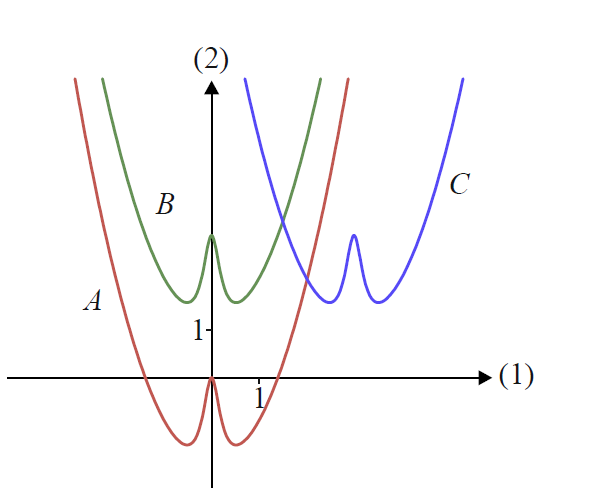
\includegraphics[scale=0.5]{Billeder/fgh.png}
\caption{Grafer for funktionerne $f,g$ og $h$.}
\label{fig:fgh}
\end{figure}
\begin{enumerate}[label=\roman*)]
\item Bestem ud fra Fig. \ref{fig:fgh} hvilken af graferne $A,B$ og $C$ der tilsvarer funktionerne $f,g$ og $h$. Begrund dit svar.
\end{enumerate}


\section*{Opgave 4 \large (med hjælpemidler) }
To linjer $l$ og $m$ i planen er givet ved henholdsvist:
\begin{align*}
&l:\  \begin{pmatrix} x\\y \end{pmatrix} = \begin{pmatrix} 7\\9 \end{pmatrix} +t\begin{pmatrix} 5\\-4 \end{pmatrix},
&m: -5x+4t+3=0.
\end{align*}
Bestem vinklerne mellem $l$ og $m$.

\section*{Opgave 5 \large (med hjælpemidler) }
For de to punkter $A(6,7)$ og $B(1,-2)$ samt vektoren $\vv{a} = \begin{pmatrix}
7\\-4
\end{pmatrix}$.
\begin{enumerate}[label=\roman*)]
\item Bestem arealet af parallelogrammet udspændt af $\vv{AB}$ og $\vv{a}$.
\item Bestem koordinatsættet til projektionen af $\vv{AB}$ på $\vv{a}$
\end{enumerate}

\section*{Opgave 6 \large (med hjælpemidler) }
Vi har to vektorer 
\begin{align*}
&\vv{v} =\begin{pmatrix}
t+7\\4
\end{pmatrix}, &&\vv{w} =\begin{pmatrix}
9t+7\\-8
\end{pmatrix}.
\end{align*}
\begin{enumerate}[label=\roman*)]
\item Bestem for hvilke værdier af $t$ det gælder, at $\vv{v}$ og $\vv{w}$ er vinkelrette.
\item Bestem for hvilke værdier af $t$ det gælder, at $\vv{v}$ og $\vv{w}$ er parallelle.
\end{enumerate}



\section*{Opgave 7 \large (med hjælpemidler) }

Vi har to vektorer 
\begin{align*}
&\vv{v} =\begin{pmatrix}
10x-3\\6
\end{pmatrix}, &&\vv{w} =\begin{pmatrix}
6\\-8x
\end{pmatrix}.
\end{align*}
\begin{enumerate}[label=\roman*)]
\item Bestem for  $x=1$ vinklen mellem $\vv{v}$ og $\vv{w}$.
\item Bestem for hvilke værdier af $x$ det gælder, at $\vv{v}$ og $\vv{w}$ er lige lange.
\end{enumerate}

\section*{Opgave 8 \large (med hjælpemidler) }
Vi har to punkter $A(0,3)$ og $B(1,4)$, samt en linje $l$ bestemt ved parameterfremstillingen
\begin{align*}
l:\ \begin{pmatrix}
x\\y
\end{pmatrix} =  \begin{pmatrix}
2\\0
\end{pmatrix}+ t \begin{pmatrix}
k^2-1\\k
\end{pmatrix},
\end{align*}
hvor $k$ er en konstant. 
\begin{enumerate}[label=\roman*)]
\item Bestem en ligning for den rette linje $m$, der går gennem punkterne $A$ og $B$.
\item Bestem $k$ så $l$ og $m$ er orthogonale.
\end{enumerate}